\begin{minipage}[b]{0.6\textwidth}
\begin{Exercise}[title = Wärmezufuhr, origin = 1. IPhO 1967, difficulty = 4, label = balls]
Die homogenen Kugeln $A$ und $B$ seien komplet identisch und haben die gleiche Anfangstemperatur. Die Kugel $A$ hängt an einem Faden von einer Decke, und die Kugel $B$ liegt auf einer horizontalen Ebene.\\
Nun wird beiden Kugeln die gleiche Menge Energie in Form von Wärme hinzugefügt, wobei sämtliche Verluste an die Umgebung vernachlässigbar seien. Wie verhalten sich die Endtemperaturen der beiden Kugeln danach?
\end{Exercise}
\end{minipage}
\begin{minipage}[t]{0.4\textwidth}
	\centering
	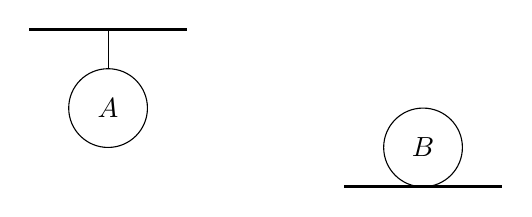
\begin{tikzpicture}
	\draw[very thick] (-4,0) -- (-2,0);
	\draw (-3,0) -- (-3,-.5);
	\draw (-3,-1) circle (.5);
	\node at (-3,-1)  {$A$};
	\draw[very thick] (0,-2) -- (2,-2);
	\draw (1,-1.5) circle (.5);
	\node at (1,-1.5) {$B$}; 
	\end{tikzpicture}
\end{minipage}